\documentclass[french]{layout/Report}
\usepackage{layout/Report}
\usepackage{layout/ReportFrontPage}

\usepackage{pgf,tikz,textcomp}
\usepackage[section]{placeins}
\usepackage{romannum}
\usetikzlibrary{arrows}
\usepackage{mathtools}
\usepackage{array}
\usepackage{color}
\usepackage{graphicx}
\usepackage{todonotes}
\usepackage{enumitem}
\usepackage{MnSymbol}

\DeclarePairedDelimiter\abs{\lvert}{\rvert}%

\begin{document}

\pagenumbering{arabic}


\frontpage{Télécommande à 1 canal par infrarouge}
%-------------------------------------------------------------------------------
\section{Introduction}
Le but est de concevoir un système d'émission - réception infrarouge avec adressage
permettant d'enclencher et déclencher un relais optique.

%-------------------------------------------------------------------------------
\section{Structure générale et principe}

On a divisé le système en 5 étages avec des interfaces définies:

\begin{description}[leftmargin=!,labelwidth=4cm, labelindent=\parindent]
\item[Générateur de signal] Générerateur de salves de N pulses de durée de 100\si{\micro\second} avec une période de 1\si{\milli\second} espacées de 100\si{\milli\second}.
\item[LED driver] Sortie de puissance qui drive la LED IR.
\item[Récepteur] Récepteur IR avec amplification et filtrage. La sortie est le signal digital des pulses.
\item[Décodeur] Circuit logique de décodage du nombre de pulses. La sortie est un pulse d'environ 5 \si{\milli\second} pour chaque salve correcte reçue.
\item[Sortie] Circuit de détection d'interruption du signal avec commutation et du relais optique.
\end{description}

\begin{figure}[h]
\centering
\vspace{5mm}
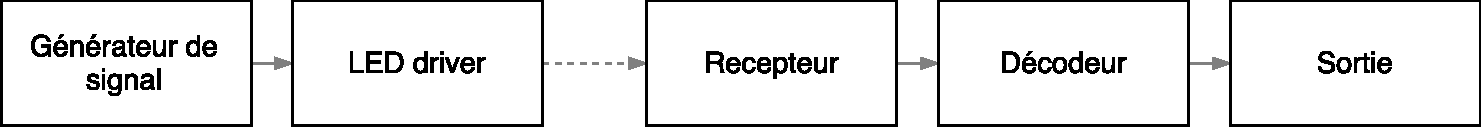
\includegraphics[width=\textwidth]{fig/IRemote_schema_structure}
% \includegraphics[width=0.8\textwidth]{fig/schema_bloc}
\caption{Schéma bloc du système avec signaux}
\label{fig:schema_bloc}
\vspace{5mm}
\end{figure}

Le but de la structure choisie est de faciliter le développement et la testabilité
du sous-système.



%-------------------------------------------------------------------------------
\section{Notation et nomenclature}

\begin{center}
	\begin{tabular}{| c | l | l |}
		\hline
		$n_{pulse}$	& Nombre de pulses dans une salve (addressage) & $13$ \\ \hline
		$t_0$				& Durée high d'un pulse	& $\SI{0.1}{\milli\second}$	\\ \hline
		$T_0$				& Période des pulse	& $\SI{1.0}{\milli\second}$	\\ \hline
		$D_0$				& Duty cycle dans une salve & $10\%$	\\ \hline
		$\tau$			& Période des slaves	& $\SI{0.1}{\second}$\\ \hline
		$t_{miss}$  & &\\ \hline
		$t_{true}$  & Durée du pulse signal une salve correcte & \\ \hline
	\end{tabular}
\end{center}

\begin{center}
    \begin{tabular}{| c | l | c |}
			\hline
        \textit{pulse}      &  \\ \hline
    \end{tabular}
\end{center}
\todo[inline]{TODO: tableau pas fini}

\subsection{Générateur de signal}
Le générateur de signal génère dans OUTPUT des salves de $n_{pulses}$ à une période $\tau$ en active high tant que celui-ci est alimenté à 3V. Les pulses dans les salves ont une durée high $t_0$ et une période $T_0$. Le nombre de pulses et les durées ne sont pas garanties lorsque l'alimentation est retirée.

\begin{description}[leftmargin=!,labelwidth=3cm, labelindent=\parindent]
	\item[Pulse timer] Génère des impulsion à hautes fréquences tant qu'il n'est pas RESET. Il est formé d'un timer TLC555 en configuration bascule astable. Les dimensionnements sont fait selon le datasheet avec une petite capacité pour la simplicité et la limitation de la consommation.
		\begin{equation*}
			\begin{cases}
				t_0 = 0.693(Rpa+Rpb)Cp \\
				T_0 = 0.693(Rpa+2Rpb)Cp \\
				Rpl	= \SI{1}{\kilo\ohm}
			\end{cases}
		\end{equation*}
	\item[Burst timer] Oscille à une période $\tau$ pour signaler le début d'une salve. Il est formé d'un timer TLC555 en configuration bascule astable. Les dimensionnements sont fait selon le datasheet avec une petite capacité pour la simplicité et la limitation de la consommation. La durée high doit être plus grand que la durée durée d'une salve.
		\begin{equation*}
			\begin{cases}
				\tau = 0.693(Rba+2Rbb)Cb \\
				n_{pulse}*\frac{T_0}{\tau} < \frac{Rba+Rbb}{Rba+2Rbb} \\
				Rbl	= \SI{1}{\kilo\ohm}
			\end{cases}
		\end{equation*}
	\item[Decounter] Compte le nombre de pulses reçu depuis son dernier RESET et signal lorsque $n_{pulse}$ pulses ont été reçu. Il est formé d'un compter HEF4526B.
	\item[Logic] Assure les conditions logiques sur les signaux. Il est formée d'un quadruple 2-input NOR HEF4001.
\end{description}

\subsection{LED driver}
Le LED driver allume la LED infrarouge lorsque LED\_SIGNAL est high. Il assure une bonne émission de la LED sans l'endommager si le signal de 3V a une période T\_0 avec un duty-cycle de 10\%.

La LED est une LD271(H). Selon son datasheet, celle-ci accepte $\SI{1}{\ampere}$ durant $\SI{0.1}{\milli\second}$ toutes les $\SI{1.0}{\milli\second}$. Ce sont ses valeurs qui ont dicté le choix du signal. Le courant est limité par la résistance $R14 = \SI{1}{\ohm}$ et une grande capacité de découplage $C7=\SI{470}{\micro F}$ assure la puissance de l'émission.


\todo[inline]{check active high/low}

\subsection{Récepteur et filtrage}

\subsection{Décodeur}
Le décodeur à 3 fonctions:
\begin{itemize}
    \item{Le comptage des pulses assuré par le \emph{decounter}. Celui-ci signal en \emph{active high} si $n_{pulse}$ ont été reçus par la tension d'entrée depuis son dernier \emph{reset}.}
    \item{La détection de pulse manquant assuré par le \emph{missing pulse detector}. Celui-ci signal en \emph{active low} si la tension d'entrée est maintenue \emph{low} pendant au moins $t_{miss} = xxx \si{\milli\second}$ après la fin d'un pulse.}
    \item{La génération du signal sortant assuré par un délais et des portes logiques. Celui si génère en \emph{active high} un pulse de $t_{true} = xx\si{\milli\second}$ si la salve est \emph{correcte}.}
\end{itemize}

Une salve est considéré correcte si le \emph{missing pulse }
\begin{center}
    \begin{tabular}{| m{4cm} | m{4cm} | l | c |}
        \hline
    % \thead{\emph{Missing pulse detector}} & \thead{\emph{Decounter}} & \thead{Statu}} & \thead{Sortie}}\ \hline
    % \thead{\emph{Missing pulse detector}} & \thead{\emph{Decounter}} & \thead{Statu} & \thead{Sortie}\\ \hline
        low     & low       & Nombre incorrect de pulses dans la salve & low \\ \hline
        low     & high  & Salve correcte    & high\\ \hline
        high    & low       & Salve non finie & low \\ \hline
        high    & high  & Salve non finie & low \\ \hline
    \end{tabular}
\end{center}

\subsection{Sortie}

\subsubsection{Détecteur de pause}
\todo[inline]{pause = lâchement de bouton, comment on veut nommer cette partie? -> Déclencheur?}

\subsubsection{Commutation de la sortie}
\subsubsection{Relais}
Le relais optique est simulé par une LED rouge standard avec un courant de 20mA et une tension directe d'environ 1.8V.
Pour alimenter la LED on a choisi le transistor bipolaire NPN BC107 avec une résistance en série pour limiter le courant.
Le BC107 a une tension \(V_{CEsat}\) de 0.25V pour un courant de 10mA.
En estimant une \(V_{CEsat}\) de 0.30V pour un courant de 20mA:
\[
R_{LED} = (5V - V_{CEsat} - V_{forward})/20mA = 145\Omega
\]
On choisit donc \(150\Omega\).

\subsection{Mesures}

Dans figure \ref{fig:decoder_signal} on voit le fonctionnement du détecteur avec différent nombres de pulses.
Dans la mesure au milieu le décodeur détecté correctement les 13 pulses et la combinaison logique
du signal du détecteur de pulse manquant et du compteur de pulses donne un signal de sortie (en vert).
Dans le cas où le mauvais nombre  de pulses (12 pulese dans la mesrue à gauche et 14 pulese à droite)
arrive à l'entrée il n'y a pas de signal à la sortie.

\begin{figure}[h]
\centering
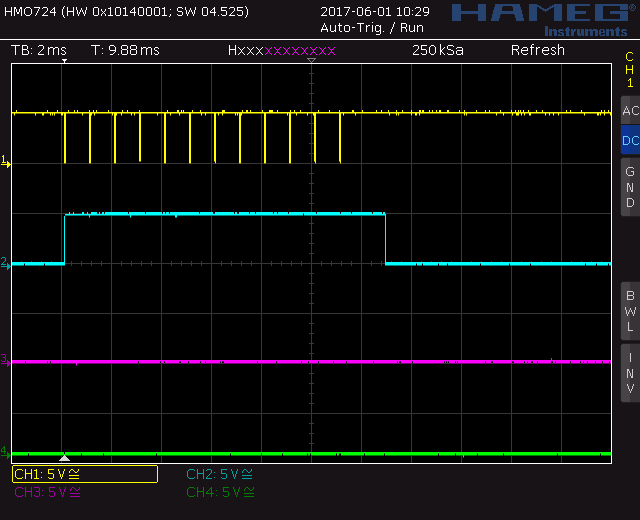
\includegraphics[width=0.3\textwidth]{../measurements/SCR06}
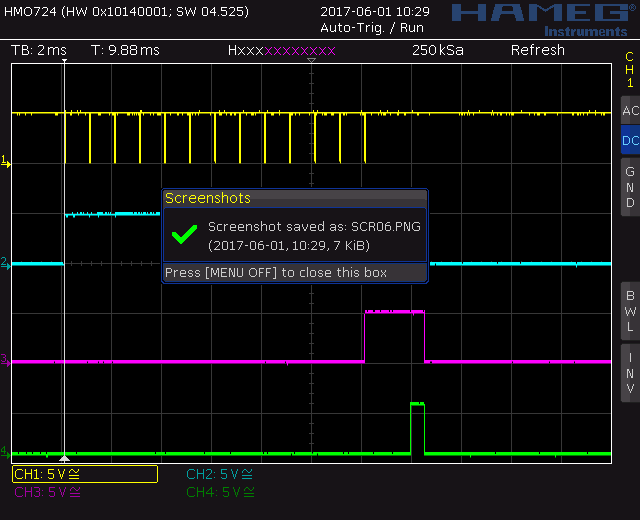
\includegraphics[width=0.3\textwidth]{../measurements/SCR07}
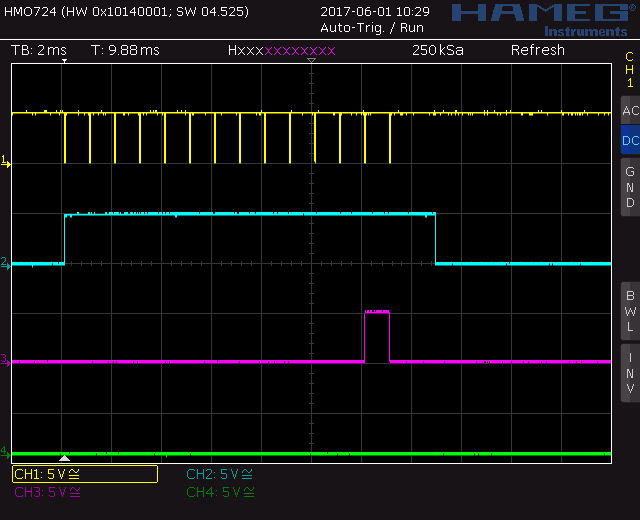
\includegraphics[width=0.3\textwidth]{../measurements/SCR08}
\caption{
\textcolor{yellow}{$\blacksquare$} Signal d'entrée,
\textcolor{blue}{$\blacksquare$} Détecteur de pulse manquant,
\textcolor{magenta}{$\blacksquare$} Compteur de pulse,
\textcolor{green}{$\blacksquare$} Sortie
}
\label{fig:decoder_signal}
\end{figure}

\begin{figure}[h]{}
\centering
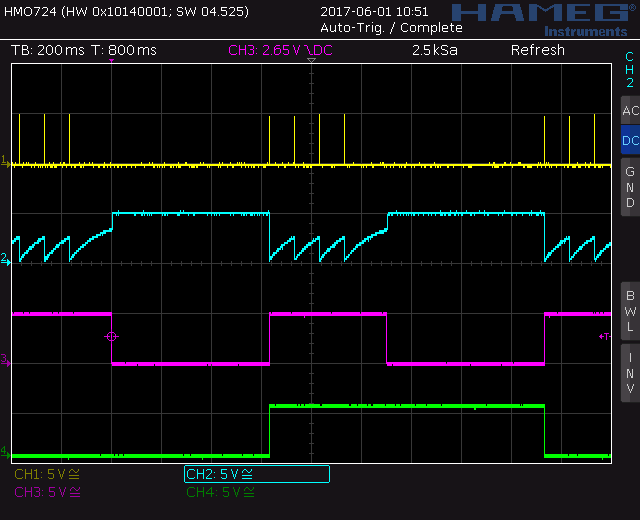
\includegraphics[width=0.3\textwidth]{../measurements/SCR12}
\caption{
\textcolor{yellow}{$\blacksquare$} Signal d'entrée,
\textcolor{blue}{$\blacksquare$} Capacité sur bascule monostable,
\textcolor{magenta}{$\blacksquare$} Sortie du détecteur de pause,
\textcolor{green}{$\blacksquare$} Sortie
}
\label{fig:output_signal}
\end{figure}

\section{Annexes}


\end{document}
